\section{Лекция 3 (24.02)}
\subsection{Структурированная расчётная сетка}
TODO
\subsection{Метод конечных разностей. Уравнение Пуассона}

\subsubsection{Постановка задачи}
Рассматривается одномерное дифференциальное уравнение вида
\begin{equation}
    \label{eq:poisson1d}
    -\ddfrq{u}{x} = f(x)
\end{equation}
в области $x\in[a,b]$ с граничными условиями первого рода
\begin{equation}
	\label{eq:poisson1d_bc}
	\begin{cases}
        u(a)=u_a,\\[5pt]
        u(b)=u_b.\\
	\end{cases}
\end{equation}

Необходимо:
\begin{itemize}
\item 
	Запрограммировать расчётную схему для численного решения этого уравнения методом конечных разностей
	на сетке с постоянным шагом,
\item
	С помощью вычислительных экспериментов подтвердить порядок аппроксимации расчётной схемы.
\end{itemize}

\subsubsection{Метод решения}

\subsubsubsection{Нахождение численного решения}

В области решения $[a,b]$ введём равномерную сетку из $N$ ячеек.
Шаг сетки будет равен $h=(b-a)/N$.
Узлы сетки запишем в виде сеточного вектора $\{x_i\}$ длины $N+1$, где $i=\overline{0,N}$.
Определим сеточный вектор $\{u_i\}$ неизвестных, элементы которого определяют значение искомого численного решения в $i$-ом узле сетки. 

Разностная схема второго порядка для уравнения \eqref{eq:poisson1d} имеет вид
\begin{equation}
    \label{eq:poisson1d_fdm}
    \frac{-u_{i-1} + 2u_{i} - u_{i+1}}{h^2} = f_i, \qquad i=\overline{1,N-1}.
\end{equation}
Здесь $\{f_i\}$ -- известный сеточный вектор, определяемый через известную
аналитическую функцию $f(x)$ в правой части уравнения \eqref{eq:poisson1d} как
\begin{equation}
    \label{eq:poisson1d_fdm2}
    f_i = f(x_i).
\end{equation}

Аппроксимация граничных условий \eqref{eq:poisson1d_bc} первого рода даёт дополнительные 
сеточные уравнения для граничных узлов
\begin{equation}
    \label{eq:poisson1d_fdm_bc}
    \begin{array}{ll}
        u_0 = u_a,\\
        u_N = u_b
    \end{array}
\end{equation}

Линейные уравнения \eqref{eq:poisson1d_fdm}, \eqref{eq:poisson1d_fdm_bc}
составляют систему вида

\begin{equation*}
    \sum_{j=0}^{N} A_{ij}\,u_j = b_i, \qquad i=\overline{0,N}
\end{equation*}
с матричными коэффициентами
\begin{equation}
    \label{eq:poisson1d_fdm_lhs}
    A_{ij} = \begin{cases}
        1,      &\quad i=0, \, j=0; \\
        2/h^2,  &\quad i=\overline{1,N-1}, \, j=i;\\
        -1/h^2, &\quad i=\overline{1,N-1}, \, j=i-1;\\
        -1/h^2, &\quad i=\overline{1,N-1}, \, j=i+1;\\
        1,      &\quad i=N, \, j=N; \\
        0,      &\quad \text{иначе}.
    \end{cases}
\end{equation}
и правой частью
\begin{equation}
    \label{eq:poisson1d_fdm_rhs}
    b_i = \begin{cases}
        u_a,   &\quad i=0;\\
        u_b,   &\quad i=N;\\
        f_i,   &\quad i=\overline{1,N-1}.
    \end{cases}
\end{equation}
Искомый вектор находится путём решения этой системы.

\subsubsubsection{Практическое определения порядка аппроксимации}
\label{sec:compute-appr}

Порядок аппрокцимации показывает скорость
приближения численного решения к точному с уменьшением сетки.
Поэтому для подтверждения порядка необходимо
\begin{itemize}
\item Знать точное решение,
\item Уметь вычислять функционал (норму, $||\cdot||$), характеризующий отклонение точного решения от численного,
\item Сделать несколько расчётов на сетках с разной $N$  и заполнить таблицу $||\{u_i - u^e(x_i)\}||(N)$,
\item На основе этой таблицы построить график в логарифмических осях и по углу наклона кривой сделать вывод о порядке аппроксимации.
\end{itemize}

Выберем произвольную функцию $u^e$ (достаточно сильно изменяющуюся на целевом отрезке $[a,b]$).

Далее путём прямого вычисления определим параметры задачи $f$, $u_a$, $u_b$ такие,
для которых функция $u^e$ является точным решением задачи \eqref{eq:poisson1d}, \eqref{eq:poisson1d_bc}.

Зададимся числом разбиений $N$ и решим задачу для выбранным параметров.
В результате определим сеточный вектор численного решения $\{u_i\}$.

В качестве нормы выберем стандартное отклонение. В интегральном виде для многомерной функции $y(\vec x)$
в области $\vec x\in D$ оно имеет вид
\begin{equation}
    \label{eq:norm2_common}
    ||y(\vec x)||_2 = \sqrt{\frac{1}{|D|}\int_{D} y(\vec x)^2 \, d\vec x}.
\end{equation}
Упрощая до одномерного случая
\begin{equation*}
    ||y(x)||_2 = \sqrt{\frac{1}{b-a}\int_{a}^{b} y(x)^2 \, dx}.
\end{equation*}

Вычислим этот интеграл численно на введённой ранее равномерной сетке $\{x_i\}$:
\begin{equation*}
    ||\{y_i\}||_2 = \sqrt{\frac{1}{b-a}\sum_{i=0}^{N} w_i y_i^2},
\end{equation*}
где $\{w_i\}$ -- вес (или "площадь влияния") $i$-ого узла:
\begin{equation*}
    w_i = \begin{cases}
        h/2, &\quad i=0, N;\\
        h, &\quad i=\overline{1,N-1},
    \end{cases}
\end{equation*}
такая что
\begin{equation*}
    \sum_{i=0}^{N} w_i = b-a.
\end{equation*}

Окончательно среднеквадратичная норма отклонения численного решения от точного запишется в виде
\begin{equation}
    \label{eq:poisson1d_fdm_norm}
    ||\{u_i - u^e(x_i)\}||_2 = \sqrt{\frac{1}{b-a}\sum_{i=0}^{N} w_i \left(u_i - u^e_i\right)^2}.
\end{equation}

\subsubsection{Программная реализация}
\label{sec:poisson1d_prog}

\clisting{open}{"test/poisson_fdm_solve_test.cpp"}

Тестовая программа для решения одномерного уравнения Пуассона 
реализована в файле \ename{poisson_fdm_solve_test.cpp}.

В качестве аналитической тестовой функции  используется
\begin{equation*}
    u^e = \sin(10 x^2)
\end{equation*}
на отрезке $x\in[0,1]$.

\subsubsubsection{Функция верхнего уровня}
объявлена как
\clisting{line}{"TEST_CASE(\"Poisson 1D solver\", \"[poisson1]\")"}
В программе в цикле по набору разбиений \cvar{n_cells}
\clisting{line}{"for (size_t n_cells"}
создаётся решатель для тестовой задачи, использующий заданное число ячеек
\clisting{line}{"worker"}
вычисляется среднеквадратичная норма отклонения численного решения от точного
\clisting{line}{"n2"}
полученное численное решение (вместе с точным) сохраняется в vtk файле\\
\ename{poisson1_n={10,20,...}.vtk}
\clisting{line}{"save_vtk"}
а полученная норма печатается в консоль напротив количества ячеек
\clisting{line}{"cout"}

В результате работы программы в консоли должна отобразиться таблица вида
\begin{shelloutput}
--- [poisson1] ---
10 0.179124
20 0.0407822
50 0.00634718
100 0.00158055
200 0.000394747
500 6.31421e-05
1000 1.57849e-05
\end{shelloutput}
где первый столбец -- это количество ячеек, а второй -- полученная для этого количества ячеек норма.
Нарисовав график этой таблицы в логарифмических осях подтвердим второй порядок аппроксимации (\figref{fig:poisson_convergence}).

\begin{figure}[h]
\centering
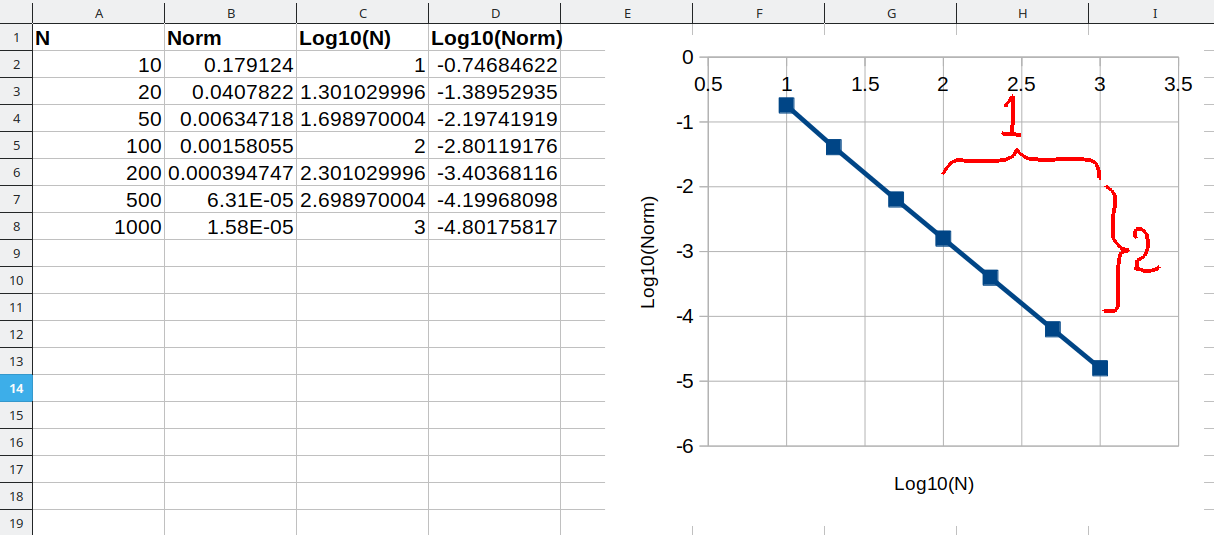
\includegraphics[width=0.9\linewidth]{poisson1_appr.png}
\caption{Сходимость с уменьшением разбиения при решении одномерного уравнения Пуассона}
\label{fig:poisson_convergence}
\end{figure}

Открыв один из cохранённых в процессе работы файлов vtk \ename{poisson1_ncells=?.vtk} в paraview
можно посмотреть полученные графики. В файле представлены как точное ``exact'', так и численное решение ``numerical''
(\figref{fig:poisson_graph}).

\begin{figure}[h]
\centering
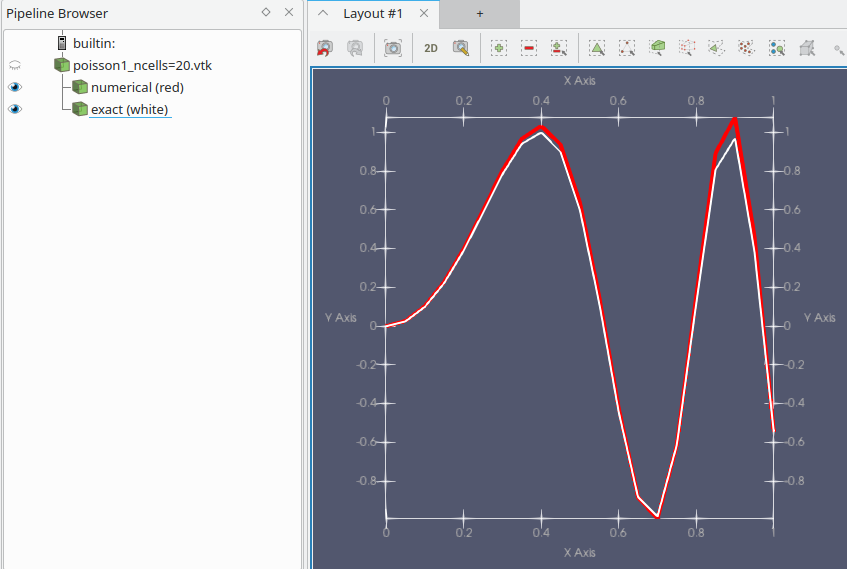
\includegraphics[width=0.9\linewidth]{poisson1_graph.png}
\caption{Сравнение точного и численного решений уравнения Пуассона}
\label{fig:poisson_graph}
\end{figure}


\subsubsubsection{Детали реализации}
\clisting{open}{"test/poisson_fdm_solve_test.cpp"}
Основная работа по решению задачи проводится в классе \cvar{TestPoisson1Worker}.

В его конструкторе происходит инициализация сетки (приватного поля класса) на отрезке $[0, 1]$ с заданным разбиением
\cvar{n_cells}:
\clisting{line}{"TestPoisson1Worker"}

В методе \cvar{solve()} производится чиленное решения задачи и вычисления нормы.
Для этого последовательно
\begin{enumerate}
\item Строится матрица левой части и вектор правой части определяющей системы уравнений.
      Матрицы хранятся в разреженном формате CSR, удобном для последовательного чтения.
\item Вызывается решатель СЛАУ. Решение записывается в приватное поле класса \cvar{u}.
\item Вызывается функция вычисления нормы.
\end{enumerate}

\clisting{block}{"double solve()"}

Функции нижнего уровня (используемые в методе \cvar{solve}):
\begin{itemize}
\item
  Сборка левой части СЛАУ. Реализует формулу \eqref{eq:poisson1d_fdm_lhs}.
  Для заполнения матрицы используется формат \cvar{cfd::LodMatrix}, удобный для непоследовательной записи, который в конце конвертируется CSR.
  \clisting{block}{"approximate_lhs("}
\item
  Сборка правой части СЛАУ. Реализует формулу \eqref{eq:poisson1d_fdm_rhs}.
  \clisting{block}{"approximate_rhs("}
\item
  Вычисление нормы. Реализует формулу \eqref{eq:poisson1d_fdm_norm}.
  \clisting{block}{"compute_norm2"}
\end{itemize}

\clearpage
\subsection{Задание для самостоятельной работы}

\subsubsection{Одномерное уравнение Пуассона}

Скомпиллировать и запустить программу, описанную в п. \ref{sec:poisson1d_prog}.
Построить график полученного численного и точного решения, аналогичный \figref{fig:poisson_graph}
(инструкцию по построению одномерного графика решения в Paraview см. в п \ref{sec:paraview-1d}).

Построить график, подтверждающий второй порядок точности
разностной схемы \eqref{eq:poisson1d_fdm}.

\subsubsection{Двумерное уравнение Пуассона}

Написать тест, аналогичный \cvar{[poisson1]}, но
для двумерной задачи на двумерной регулярной сетке
\begin{equation*}
   -\left(\dfrq{u}{x} + \dfrq{u}{y}\right) = f(x, y).
\end{equation*}
использовать разностную схему
\begin{equation*}
   \frac{-u_{k[i-1,j]} + 2 u_{k[i, j]} - u_{k[i+1,j]}}{h_x^2} +
   \frac{-u_{k[i,j-1]} + 2 u_{k[i, j]} - u_{k[i,j+1]}}{h_y^2} =
   f_{k[i,j]},
\end{equation*}
где
\begin{equation}
    \label{eq:tasks_ij2k}
    k[i, j] = i + (n_x+1) j
\end{equation}
-- функция, переводящая парный $(i,j)$ индекс узла регурярной сетки ($i$) для оси x, $j$ для оси y) в сквозной индекс $k$
сеточного вектора, $n_x$ -- количество ячеек сетки в направлении x.

При вычислении весов $w_k$ для вычисления среднеквадратичного отклонения учесть
наличие граничных и угловых точек:
\begin{equation*}
    w_k = \begin{cases}
            h_x h_y / 4,  &\quad  \text{для угловых точек};\\
            h_x h_y / 2,  &\quad  \text{для граничных неугловых точек};\\
            h_x h_y,      &\quad  \text{для внутренних точек}.
    \end{cases}
\end{equation*}
Четрые угловые точки определяются как
\begin{equation*}
    i[k], j[k] = (0, 0), \, (0, n_y), \, (n_x, n_y), \, (n_x, 0)
\end{equation*}
Граничные неугловые точки:
\begin{equation*}
    \begin{array}{lll}
        i[k], j[k] =& \overline{1,n_x-1}, 0;    & \text{нижняя сторона},\\
                    & n_x, \overline{1,n_y-1};  & \text{правая сторона},\\
                    & \overline{1, n_x-1}, n_y; & \text{верхняя сторона},\\
                    & 0, \overline{1,n_y-1};    & \text{левая сторона}.
    \end{array}
\end{equation*}
Функции, переводящие сквозной индекс в пару $i,j$, имеют вид
\begin{equation}
    \label{eq:tasks_k2ij}
    \begin{array}{ll}
        i[k] = {\rm mod}\left(k, \left(n_x+1\right)\right), & \text{// остаток от деления},\\
        j[k] = \lfloor k / \left(n_x+1\right)\rfloor,       &\text{// целая часть от деления}.\\
    \end{array}
\end{equation}

Использовать класс \cvar{cfd::RegularGrid2D} для задания сетки.
Функции перевода индексов узлов из сквозных в парные и обратно реализованы в классе двумерной регулярной сетки:
\begin{itemize}
\item \cvar{cfd::RegularGrid2D::to_split_point_index}
\item \cvar{cfd::RegularGrid2D::to_linear_point_index}
\end{itemize}

В случае, если решатель системы линейных уравнений не решает построенную матрицу, использовать функцию
\cvar{cfd::dbg::print} для отлаточной печати матрицы в консоль (размерность задачи должна быть небольшой).

Для иллюстрации двумерного решения в Paraview использовать изолинии (\ref{sec:paraview-isolines}) и трёхмерные поверхности (\ref{sec:paraview-2d}).

Построить график сходимости для двумерного случая.
Следует иметь ввиду, что на графике сходимости
по оси абсцисс отложено линейное разбиение, вычисляемое как
$n=\sfrac{1}{h}$, где $h$ -- это характерный линейный размер ячейки.
Для двумерных сеток этот линейный размер
сетки можно вычислить через среднюю площадь ячейки $A$ как $h = \sqrt{A}$,
которую в свою очередь можно получить, разделив общую площадь на количество
ячеек: $A = \sfrac{|D|}{N}$. Тогда, в случае единичного квадрата, линейное разбиение будет равно $n = \sqrt{N}$.
